\documentclass[UTF8, twoside]{EPURapport}
\usepackage{algpseudocode}
\usepackage{algorithm}
\usepackage{pdfpages}
\usepackage[nottoc, notlof, notlot]{tocbibind}
\usepackage{amsmath,amsfonts,amsthm}
\usepackage{graphicx}
\usepackage{rotating}
\usepackage{color}
\usepackage{colortbl}
%\usepackage{listings}

%\renewcommand{\lstlistlistingname}{Liste des codes}
%\renewcommand{\lstlistingname}{Code}

%\addextratables{%
%	\lstlistoflistings
%}

%\swapAuthorsAndSupervisors



\thedocument{Operational research project draft}{Ant colony optimization algorithm for a combined routing and scheduling problem}{Ant colony optimization algorithm for a combined routing and scheduling problem}

\grade{Computer Aided Decision Support\\ International Research Master 2\\ 2013 - 2014}

\authors{%
	\category{Student}{%
		\name{Thomas NOGUER} \mail{thomas.noguer@etu.univ-tours.fr}
	}
	\details{M2RI CADS 2013 - 2014}
}

\supervisors{%
	\category{Supervisors}{%
		\name{Jean-Charles BILLAUT} \mail{jean-charles.billaut@univ-tours.fr}
		\name{Nicolas MONMARCHÉ} \mail{nicolas.monmarche@univ-tours.fr}
	}
	\details{Université François-Rabelais, Tours}
}

\abstracts{abstract}
{keywords}

\begin{document}

\chapter{Formalization of the problem}

	The problem can be defined from three differents subproblems :
	
\begin{itemize}
\item[$\bullet$] The two machines permutation flowshop. We have two machines $M_1$ and $M_2$ organized as a flowshop. A set of $n$ jobs have to be scheduled into a sequence. Each job $j$ has a value $a_j$ and $b_j$ that correspond to the time required to complete the job $j$ on $M_1$ and $M_2$ respectively.
\item[$\bullet$] The grouping of jobs to be delivered. When the jobs are completed for the two machines permutation flowshop we must form groups of jobs, where a group must contain at least one job. These groups are then used for the third subproblem.
\item[$\bullet$] A traveling salesman problem. We consider one truck taking the group of jobs previously formed where each job has a destination $k_j$. The idea is to find the sequence of destinations in order to deliver every job from the group while minimizing the traveling distance. We have a matrix $K$ ($m \times m$) where $m$ is the number of destinations and $K_i^j$ is the distance between the destination $i$ and $j$.
\end{itemize}

	The objective function is to minimize the sum of lateness of the jobs $\overset{j \leq n}{\underset{j=1}{\sum}} L_j$. The lateness $L_j$  of a job $j$ is the difference between the completion time of the job $c_j$ and its due date $d_j$: $L_j = c_j - d_j$. The completion time of a job is not equal to the completion time of the job for the flowshop problem but for the traveling salesman problem. \textbf{$c_j$ is equal to the date at which the truck is coming back to the factory after its deliveries.}
\textbf{We consider that the truck has no capacity limit, it can carry has many jobs has possible.}
\\

	The input data of our problem are the following :
\begin{itemize}
\item[$\bullet$] The number $n$ of jobs,
\item[$\bullet$] The values $a_j$, $b_j$ and $d_j$ of job $j$ ($\forall j \in [1,n]$),
\item[$\bullet$] The number of $m$ destinations,
\item[$\bullet$] The destination $k_j$ of job $j$ ($\forall j \in [1,n]$),
\item[$\bullet$] The matrix $K$ ($m \times m$) of distances between each destination.\\
\end{itemize}

	During the resolution of the problem we must find the sequence of jobs on the flowshop, the groups of jobs to be delivered and the sequence of delivery for each group.

	We proposed a first way of encoding a solution : a table of size $n$ containing the sequence of job for the flowshop subproblem, a table of size $2n$ containing the groups and sequences for the traveling salesman subproblem. The first cell of the second table contains the number of jobs for the first group, the following cells contain the number of jobs in the delivery sequence and so on. The figure \ref{problem} shows a solution for a simple instance of the problem with its encoding. 
	
	The sequence here is $\{1,2,3\}$ the first group $G_1$ of jobs is $G_1 = \{1,2\}$ and 1 is delivered first, the second group $G_2$ only contains one job $G_2 = \{3\}$.
	
	
\begin{figure}
	\centering 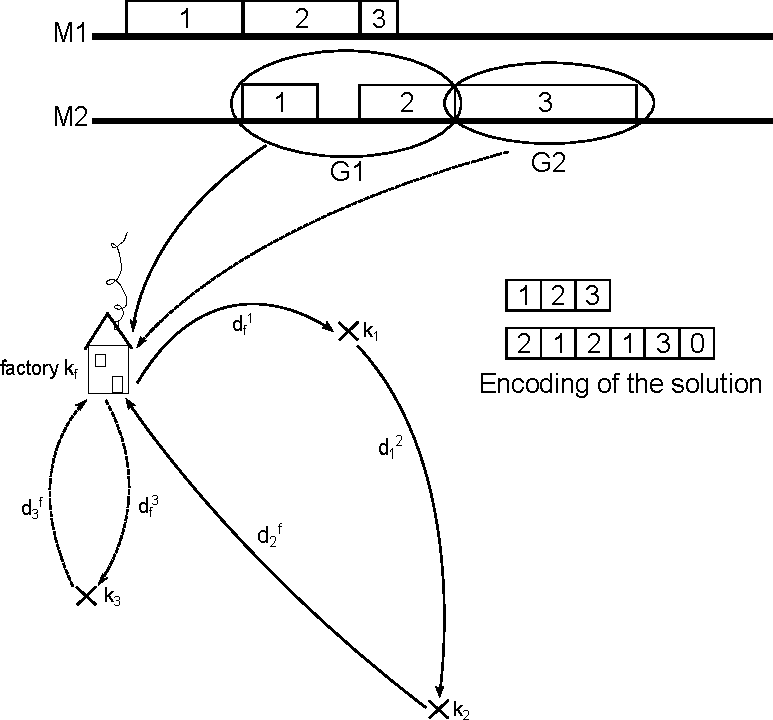
\includegraphics{images/problem.pdf}
	\caption {A solution of the problem for a simple instance}	
	\label {problem}
\end{figure}

\chapter{Ant colony optimization}

\section{General definitions}

 	\hspace{4ex}In this first part we will consider a traveling salesman problem in order to explain the mecanism of the ant colony metaheuristic. The graph representation of cities is an intuitive approache for such a method.
	
	
	The classic algorithm of an ant colony heuristic is the following :

\begin{algorithm}
  \caption{Ant colony}
  \begin{algorithmic}[1]
      \For{$k \gets 1 \textrm{ to } iterationsNumber$}
      	\For {\textbf{each} $ant$}
        	\State Construct solution
			\State Local pheromone update
        \EndFor
        \State Local search
        \State Global pheromone update
      \EndFor
      \State \textbf{return} Best found solution
  \end{algorithmic}
\end{algorithm}

	In order to construct we need to use a probability formula based on the following :
	\\

\[
P^m_{}ij= \left\{ 
\begin{array}{l r}
\frac{[\tau_{ij}]^\alpha \cdot [\eta_{ij}]^\beta}{\underset{l\notin tabu_m}{\sum}[\tau_{il}]^\alpha \cdot [\eta_{il}]^\beta} & \text{if } j\notin tabu_m\\
0 & \text{if } j\in tabu_m
\end{array}
\right.
\]

	Where $P^m_{ij}$ is the probability of an ant $m$ in city $i$ to go to the city $j$, $\tau{ij}$ the intensity of the pheromone trail from $i$ to $j$, $\eta_{ij}$  the visibility of city $j$ from city $i$ (this is typically $1/d_{ij}$ where $d_{ij}$ is the distance between $i$ and $j$). $\alpha$ and $\beta$ are parameters used to make the pheromone trail of the visibility more important from one another. And finally, the tabu list is used to prevent ants from going to forbidden cities like the city they come from.
\\

	The local pheromone update is used to emulate the evaporation phenomenom of pheromone. This evaporation is calculated from a formula based on the following :
	\\
	
\[
\tau_{ij} = (1-\rho) \cdot \tau_{ij}+\rho \cdot \tau_{min}
\]

	Where $\rho$ is the evaporation rate and $\tau_{min}$ the minimum value of the pheromone trail, which is also usualy used as initial value. \textbf{It is important to consider that the evaporation function is only used for the paths the ants traveled through.}
\\

	The global pheromone update is used to emulate the deposit of pheromone from the ants. This deposit is calculated from a formula based on the following :
	\\
	
\[
\tau_{ij} = (1-\rho) \cdot \tau_{ij}+\rho \cdot \Delta\tau_{ij}
\]

	Where $\Delta\tau_{ij}$ can be defined as follows :
	\\
	
\[
\Delta\tau_{ij} = \left\{ 
\begin{array}{l l}
15 & \text{if } (i,j) \text{ is an edge in the best and second best,}\\
10 & \text{if } (i,j) \text{ is an edge only in the best,}\\
5 & \text{if } (i,j) \text{ is an edge only in the second best}\\
\end{array}
\right.
\]

\section{Application to the combined routing and scheduling problem}

	\hspace{4ex}One main issue to overcome here is the fact that there is no simple graph representation of the complete problem. For the traveling salesman problem, it is easy to see how the pheromone trails and the visibility comes from. For our problem it is quite different. We can try to imagine a graph that an ant could visit and form a complete solution from it. For instance, a node could represent the fact that a job $j$ is placed first in the flowshop, alone in a delivery group and delivered first. But we then have to consider every possibility knowing that the grouping and delivering problems are dependant on the flowshop. If we change the sequence of jobs in the flowshop we obtain a different grouping problem and then a different traveling salesman problem.
	
	Even though we happen to be able to model such graph, its size would be unreasonably huge. It is not rational to chose such solution. \textbf{We must abandon the idea to apply the ant colony optimization all at once for our problem, we need to think of a different approach.}
	\\
	
	Instead of trying to use the ant colony metaheuristic for the complete problem, we can consider using it for parts of it. \textbf{We can chose to use the ant colony on one or several subproblem and use different method to contruct the rest of the solution and then update the pheromone trails based on the results of the whole solution.} 
	
	Although is not clever to consider using the ant colony for the traveling salesman subproblem since the problem is different each time you change the groups to be delivered or the sequence of jobs from the flowshop. The pheromone trails would be lost each time you change the solution in any subproblem above.
	
	We can still consider the other two subproblems as potential candidate for the ant colony. Indeed, the flowshop problem and the grouping problem can both be considered central in our global problem. \textbf{We then have three posibilities, use the ant colony on the flowshop, on the grouping problem or both and use simple heuristics coupled with a surrogate mecanism to obtain the value of the objective function for our solution in order to guide the ants towards the best solution.} The surrogate mecanism could be very useful in order to save time computation, it would be used in the majority of cases and replaced with heuristics in the others in order to verify if the current solution is still a good one.
	
\end{document}
